\chapter{Adversarios Clasificadores}



Los adversarios clasificadores son programas de c\'omputo que se dedican a observar  mensajes que se intercambian  entre  los  usuarios  de  correo  electrónico,  con  el  fin  de  clasificarlos  e 
identificar  a  todos  los  usuarios  que  cumplan  con  cierto  criterio.  Esta  clasificación  se hace de manera masiva a trav\'es de  una búsqueda de palabras clave dentro de 
los  mensajes de  los usuarios. Por ejemplo, el  clasificador puede estar interesado en  los mensajes  que  contienen  la  palabra  clave  "Bomba",  así  que 
todos  los  mensajes  que contengan esta palabra serán etiquetados en una clasificación en específico, este proceso se lleva a cabo por medio de técnicas de 
“Reconocimiento de patrones” y “Aprendizaje Máquina” para encontrar y clasificar los mensajes 
que intercepta~\cite{clas,Attacks}.
\\
La  clasificación  de  estos  mensajes  tiene  diversos  usos, ya  que  pueden  ser  clasificados con  fines demográficos, con  fines comerciales o con  fines gubernamentales. Todo esto 
con  el  propósito  de  generar  las  estadísticas  de  comportamientos  e  intereses  de  los usuarios de correo electrónico. \\




En este trabajo terminal, se considera que un adversario clasificador solo es capaz de realizar ataques de solo texto cifrado (ciphertext only attack, en ingl\'es). Como se mencion\'o en el cap\'itulo anterior, en este ataque  el adversario solo  cuenta  con  los  textos  cifrados  que  va  recopilando  de  un  canal  o  base  de 
datos. Posteriormente, el adversario utiliza  estos  textos  cifrados  para  hacer  un  análisis  criptográfico  de  cómo  se comporta la técnica de cifrado  y tratar de hallar el texto en claro a partir de los textos cifrados que va recopilando. 
\\
Este  tipo  de  ataques  es  muy  común  en  el  internet  aunque  con  muy  baja  efectividad cuando   se   implementa   en   comunicaciones   altamente   protegidas,   y   cuando   se 
implementa en canales de comunicación desprotegidos  la  información obtenida  llega  a ser  muy  pobre.  En  los  últimos  años  se  han  dado  cuenta  que  si   este  tipo  de 
adversarios   atacan las  comunicaciones  sin  cifrado se  obtienen  características  valiosas  sobre  los usuarios  que  utilizan  este  tipo  de  canales  de  comunicación,  este  tipo  de  ataques  son 
ejecutados por  adversarios clasificadores.\\


\subsection{Esquema Golle - Farahat}
La  única  referencia  que se tiene  sobre  un  esquema  criptográfico  contra  adversarios clasificadores es el que propusieron Golle y Farahat~\cite{Attacks}. En este art\'iculo se habla por primera vez de las caracter\'isticas de este tipo de adversarios  y se considera la posibilidad de utilizar un esquema de cifrado con un nivel de seguridad menor.
%en el artículo 
%“Defending Email Communication Against Profiling” de Philippe Golle  y  Ayman  Farahat, ambos  miembros del 
%“Palo Alto Research Center”.\cite{Attacks}\\
%En su artículo se aborda el ataque de adversarios clasificadores sobre los mensajes de correo electrónico, en el cual se proponen un protocolo para la comunicación por correo electrónico. 
Golle y Farahat proponen un protocolo que hace uso de una función  de cifrado, el cual sustituye cada una de las palabras del mensaje por otra de la misma extensión y frecuencia gramatical, esta función esta pensada para textos en idioma ingl\'es. 
%Esta función tiene como parámetro una clave $K$.  
Para cifrar se utiliza una clave que se genera  usando los datos de cabecera que acompañan al mensaje los cuales pueden ser dirección  del remitente, la dirección del destinatario, la hora a la que se envía el correo electrónico y potencialmente otros campos. Estos datos se introducen en una función hash lenta y el resultado de esta función es la clave $K$. Estas funciones hash  tiene con una complejidad de c\'alculo moderadamente mas alta que las 
funciones hash est\'andar.  \\
Este  protocolo resulta inseguro para la criptografía moderna pero es efectivo contra el ataque de clasificadores. Por otro lado este protocolo resuelve dos problemas, le  permite  a los usuarios  calcular  la  clave de cifrado y descifrado  fácilmente  ya  que  los datos del mensaje con que se calcula son  públicos, resolviendo así el intercambio de claves. Al usar un cifrado de tipo semántico se permite que el texto se vea como un texto en inglés pero indistinguible para los clasificadores y por lo tanto este clasifica incorrectamente el mensaje cifrado.\\

\section{CAPTCHA}
 Es un programa informático diseñado para diferenciar un ser humano de una computadora, CAPTCHA son las siglas de prueba de Turing completamente automática y pública para diferenciar computadoras de humanos ({\it Completely Automated Public Turing test to tell Computers and Humans Apart} por sus siglas en ingl\'es).  Un CAPTCHA es una prueba que es fácil de pasar por un usuario humano pero difícil de pasar por una máquina. Uno de los CAPTCHAs más com\'unes son imágenes distorsionadas de cadenas cortas de caracteres. Para un humano es generalmente muy fácil recuperar la cadena original de la imagen distorsionada, pero es difícil para  los algoritmos de reconocimiento de caracteres recuperar la cadena original de la imagen distorsionada.\\
Un CAPTCHA en un algoritmo aleatorio $G$, que recibe como parámetro una cadena de caracteres STR y produce como resultado un CAPTCHA $G(x)$\\

\begin{figure}[H]
\centering
	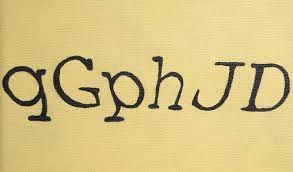
\includegraphics[width=5cm, height=3cm]{./images/cptc.jpeg}
	\caption{CAPTCHA}
	\label{fig:3-6}
\end{figure}
 
%La criptografía moderna se basa en dos corrientes metodológicas que son la criptografía simétrica  y  la criptografía asimétrica. Estas dos técnicas tienen como propósito ocultar 
%el  contenido  de  un  mensaje  con  el  fin  de  que  solo  sea  leído  por  aquellos  que  estén autorizados, a esto se le llama cifrado. 




\section{Esquema de Secreto Compartido de Shamir}
El esquema de secreto compartido fue propuesto por Adi Shamir en 1997\cite{shamir}. 
El objetivo de este método es dividir un secreto $K$ en $w$ partes,que son dadas a $w$ participantes. Para recuperar el secreto es necesario tener al menos $u$
elementos de las $w$ partes siendo $u \leq w$. Y no es posible recuperar el secreto si se tienen menos que $u$ partes.

Para construir el esquema del secreto compartido primero es necesario seleccionar un número primo $p \geq w+1$ el cual define al conjunto $\mathbb{Z}_p$.
\\
\\
El procedimiento para dividir un secreto $K$ en $w$ partes es el siguiente:

\begin{enumerate}
 \item Se seleccionan $w$ elementos distintos de cero del conjunto $\mathbb{Z}_p$ denotados como $x_i$ donde $1 \leq i \leq w$.
 \item Se seleccionan $u-1$ elementos aleatorios de $\mathbb{Z}_p$ denotados como $a_1,...,a_{u-1}$.
 \item Se construye el polinomio $y_x$ de la siguiente forma. Sea \begin{equation}
            y(x)=K+\sum_{j=1}^{u-1} a_j x^j \bmod \quad p
           \end{equation}
           Por medio de este polinomio se calculan los elementos $y_i$.
 \item La salida es el conjunto $S=\{(x_1,y_1),...,(x_w,y_w)\}$.
\end{enumerate}

Para recuperar el secreto solo tenemos que resolver un sistema de ecuaciones  que es definido por el polinomio característico $a(x)=a_0+a_1x+...+a_{u-1}x^{u-1}$.
\\
\\
Posteriormente se seleccionan $u$ pares de elementos $(x_w,y_w)$ con los que obtendremos nuestro sistema de ecuaciones a resolver. El elemento que nos interesa obtener del sistema de ecuaciones es $a_0$ ya que este es el valor de nuestro secreto $K$.
\begin{example}
Si se considera el conjunto  $\mathbb{Z}_{11}$ y se desea compartir el secreto $K=8$, entre 5 participantes,
de tal manera que solo cuando se re\'unan cualesquiera 2 de ellos sea posible recuperar $K$, es decir
 $w=5$ y $u=2$.

Se seleccionan los $u-1$ elementos del conjunto $\mathbb{Z}_{11}$, puesto que $u=2$ en este caso solo 
hay que escoger un elemento: $a_1=5$.

A continuaci\'on se seleccionan $w$ elementos de $\mathbb{Z}_{11}$, por ejemplo 
 $x_1=2, x_2=7, x_3=9, x_4=10, x_5=3$.

Posteriormente, se calcula el conjunto de elementos $y_i$ por medio de la ecuaci\'on 
\begin{equation} \nonumber
 y_i=k+\sum_{j=1}^{u-1} a_j x_i^j \bmod \quad p
\end{equation}

En el caso del ejemplo, la ecuaci\'on anterior queda como sigue:

\begin{equation} \nonumber
 y_i=K+a_1x_i \bmod \quad p
\end{equation}
Y se obtienen los siguientes valores:
$$\begin{array}{lcl}
y_1&=&8+5(2) \bmod 11=7, \\
y_2&=&8+5(7) \bmod 11=10,\\
y_3&=&8+5(9) \bmod 11=9, \\ 
y_4&=&8+5(10) \bmod11=3, \\
y_5&=&8+5(3) \bmod 11=1. 
\end{array}$$

Finalmente, se tienen los pares $S=\{ (2,7), (7,10), (9,9), (10,3),(3,1)\}$
%$A_1(2,7)$\hspace{1cm}$A_2(7,10)$\hspace{1cm}$A_3(9,9)$\hspace{1cm}$A_4(10,3)$\hspace{1cm}$A_5(3,1)$\\


Para recuperar la llave $K$ es necesario seleccionar $u=2$ pares del conjunto $S$, por ejemplo
$A_2(7,10)$, $A_4(10,3)$. Con estos pares se puede crear el siguiente  sistema de ecuaciones:
$$\begin{array}{lcl}
 a_0+a_1x_2&=&y_2 \\
 a_0+a_1x_4&=&y_4 
 \end{array}$$
 Es importante notar, que en tal sistema de ecuaciones, las inc\'ognitas son $a_0$ y $a_1$, las cuales
 son desconocidas para los $w$ participantes.  Para el esquema de secreto compartido de
 Shamir, es de particular inter\'es $a_0$, ya que  $a_0=K$.
Al sustituir los pares $A_2$ y $A_4$ en el sistema de ecuaciones anterior, se tiene:
\begin{align}
a_0+7a_1&=10 \label{eq-3}\\
a_0+10a_1&=3 \label{eq-4}
\end{align}
Para resolver este sistema se puede utilizar cualquiera de los métodos com\'unes que se usan en álgebra, solo que respetando el conjunto $\mathbb{Z}_p$, en este caso se resolverá por el método suma y resta.\\
%\begin{equation*}
% a_0+7a_1=10
%\end{equation*}
%\begin{equation}
% a_0+10a_1=3
%\end{equation}
Multiplicamos la ecuación~(\ref{eq-3}) por $-1$ y obtenemos:
\begin{equation}
 -a_0-7a_1=-10 \label{eq-5}
\end{equation}
%\begin{equation}
% a_0+10a_1=3
%\end{equation}
sumamos la ecuación~(\ref{eq-4}) con (\ref{eq-5})  d\'andonos como resultado:
\begin{equation} \nonumber
 3a_1=4
\end{equation}
de donde es posible despejar$a_1$
\begin{equation}
 a_1=\frac{4}{3} \label{eq-8}
\end{equation}
Puesto que 4 es el inverso multiplicativo de 3,  la ecuación~(\ref{eq-8}) queda de la siguiente forma
\begin{equation} \nonumber
 a_1=(4)(4)=16 \bmod 11 =5
\end{equation}
Sustituimos $a_1$ en la ecuación~(\ref{eq-4}) 
\begin{equation} \nonumber
 a_0+10(5)=3
\end{equation}
Simplificamos y despejamos $a_0$
\begin{align*}
 a_0+(50 \bmod 11)=3 \\
  a_0=-3 \bmod11=8
\end{align*}
Como $a_0=8$ podemos ver que se recuper\'o a $K$ exitosamente ya que  $a_0=K$.
\end{example}


\section{Esquema Díaz - Chakraborty}
Otro esquema para combatir a los adversarios clasificadores fue propuesto en 2012 por D\'iaz y 
Chakraborty~\cite{clas}.  El esquema D\'iaz-Chakraborty utiliza CAPTCHAs y un algoritmo de clave secreta,
para  proteger el correo electr\'onico. 
 Para obtener la clave se genera una cadena al azar, a la se le aplica una funci\'on hash, con esta clave se cifra el
 mensaje.  Tanto el mensaje cifrado como el CAPTCHA se env\'ian al receptor. El receptor debe
resolver el CAPTCHA, para obtener la cadena, aplicarle la funci\'on hash y as\'i obtener la clave de cifrado. Puesto que un adversario clasificador es un programa de c\'omputo, no podr\'a resolver un CAPTCHA y por tanto no podr\'a obtener la clave de cifrado.  Este esquema se muestra en la Figura~\ref{fig:protocol}.

\begin{figure}[h]
\centering
%\subfigure{
\begin{tabular}{|l|}
\hline
\begin{minipage}{220pt}
\begin{tabbing}
\ \ \ \ \ \=\ \ \ \ \=\ \ \ \ \=\ \ \ \ \=\ \ \ \ \=\ \ \ \ \=\ \ \
\ \kill \\
\ \ \ \ {\bf Protocol} ${\mathbb P}(x)$\\
\> 1. \> $k\rand {\sf STR}$; \\
\> 2. \> $k^{\prime} \leftarrow G(k)$; \\
\> 3. \> $K \leftarrow H(k)$; \\
\> 4. \> $c\leftarrow E_K(x)$;\\
\> 5. \> {\bf return} $(c, k^{\prime})$
\end{tabbing}
\end{minipage}\\
\hline
\end{tabular}
\caption{\label{fig:protocol} Protocol D\'iaz-Chakraborty.}
\end{figure}

 
%\begin{enumerate}
% \item \textbf{Esquema P}: Se genera una cadena de caracteres aleatoriamente llamada STR la cual es introducida a una funcion Hash para generar la clave $K$, con esta clave se cifra el mensaje original $M$. La cadena STR es convertida en un CAPTCHA y se envía junto con el texto cifrado al destinatario.\\\\
% \textbf{Esquema} P(x)
% \begin{enumerate}
%  \item $k\longleftarrow^\$ STR;$
%  \item $k'\longleftarrow G(k);$
%  \item $K\longleftarrow H(k);$
%  \item $c\longleftarrow E_k(x);$
%  \item $return(c,k')$
% \end{enumerate}
 Contemplando que es muy común que el usuario no consiga resolver el CAPTCHA D\'iaz y Chakraborty propusieron una variante del esquema anterior, el cual se describe a continuaci\'on. 
 Se genera una cadena de caracteres aleatoriamente llamada STR la cual se codifica a un valor entero. El valor entero es dividido en 5 pares $(x,k')$ por medio del algoritmo de Secreto Compartido, cada uno de los elementos $k'$ de los pares generados es decodificado a su correspondiente valor en cadena de caracteres para posteriormente ser convertidos en CAPTCHAS. Para finalizar la cadena STR se introduce en una función Hash para generar la llave $K$. Con esta llave se cifra el mensaje de correo y se envía junto con los pares de $(x,CAPTCHA)$.
Este esquema se puede observar en la Figura~\ref{fig:P-with-sharing}.
\begin{figure}[h]
\begin{center}
\begin{tabular}{|l|}
\hline
\begin{minipage}{220pt}
\begin{tabbing}
\ \ \ \ \ \=\ \ \ \ \=\ \ \ \ \=\ \ \ \ \=\ \ \ \ \=\ \ \ \ \=\ \ \
\ \kill \\
\ \ \ \ {\bf Protocol} ${\mathbb P}^{\prime}(x)$\\
\> 1. \> $k\rand {\sf STR}$; \\
\> 2. \> $k^\prime \leftarrow {\sf ENCD}(k,0);$\\
\> 3. \> $\{ (x_1, k_1^\prime), \ldots, (x_w, k_w^\prime)\} \leftarrow {\sf SHARE}^p_{u,w}(k^\prime)
$; \\
\> 4. \> {\bf for} $i=1$ {\bf to } $w$; \\
\> 5. \>\> $(k_i, \lambda_i) \leftarrow {\sf ENCD}^{-1}(k_i^\prime)$; \\
\> 6. \>\> $c_i \leftarrow G(k_i)$; \\
\> 7. \>{\bf end for} \\
\> 8. \> $K \leftarrow H(k)$; \\
\> 9. \> $C\leftarrow E_K(x)$; \\
\> 10. \> \hspace*{2mm}{\bf return} $[C,\{ (x_1, c_1, \lambda_1), \ldots, (x_w,
c_w, \lambda_w)\}]$
\end{tabbing}
\end{minipage}\\
\hline
\end{tabular}
\end{center}
\caption{\label{fig:P-with-sharing} Variante del  protocolo D\'iaz-Chakraborty}
\end{figure} 


% \begin{enumerate}
%  \item $k\longleftarrow^\$STR;$
%  \item $k'\longleftarrow ENCD(k);$
%  \item $\{(x_1,k'_1),...,(x_w,k'_w)\}\longleftarrow SHARE^p_{u,w}(k');$
%  \item $for\quad i=1\quad to \quad w;$
%  \item $\quad (k_i)\longleftarrow ENCD^{-1}(k'_1);$
%  \item $\quad c_i\longleftarrow G(k_i);$
%  \item $end for$
%  \item $K\longleftarrow H(k);$
%  \item $C\longleftarrow E_k(x);$
%  \item $return [C,\{(x_1,c_1),...,(x_w,c_w)\}]$
% \end{enumerate}


Este nuevo esquema se cre\'o pensando en que el usuario pueda tener más oportunidades de recuperar el mensaje cifrado y esto sucede gracias a el algoritmo de Secreto Compartido, ya que no este podemos tener la misma llave repartida en $n$ CAPTCHAS. A continuaci\'on se describe las funciones {\sf ENCD} y ${\sf ENCD}^{-1}$, cuyo
prop\'osito es convertir una cadena de caracteres a enteros y viceversa. 

\subsection{Codificaci\'on de caracteres a enteros}
Se tiene un conjunto de caracteres $AL$ compuesto por $AL=\{A,B,...,Z\}\cup\{a,b,...,z\}\cup\{0,1,...,9\}\cup\{+,/\}$ con una cardinalidad $|AL|=64$.

Para obtener una representación binaria de 64 elementos son necesarios 6 bits por lo que para todos los elementos $\sigma\epsilon AL$ existe una cadena binaria. Una vez establecido esto el procedimiento para realizar la conversión es el siguiente:
\begin{enumerate}
 \item Tomamos una cadena de caracteres y la separamos caracter por caracter y los intercambiamos por su correspondiente número entero en $AL$ $\alpha _0||\alpha _1||...||\alpha _m$
 \item Posteriormente cada uno de los enteros lo convertimos en un binario de 6 bits y se concatenan uno detrás del otro $\Psi\longleftarrow bin_6(\alpha _0)||bin_6(\alpha _1)||...||bin_6(\alpha _m$
 \item La cadena binaria $\Psi$ la convertimos a entero $v\longleftarrow toInt(\Psi)$
\end{enumerate}
\textbf{Ejemplo}:\\
Tenemos la cadena $STR=`ABC`$ de la cual cambiaremos cada caracter por su correspondiente valor entero en $AL$ quedando de la siguiente manera $\alpha =\{0,1,2\}$
\\ 
\\
Ahora cada  uno de los elementos de $\alpha$ lo convertiremos a su correspondiente representacion binaria, $bin_6(0)=000000, bin_6(1)=000001, bin_6(2)=000010$ y concatenamos cada una quedando $\Psi = 000000000001000010$. 


La cadena binaria $\Psi$ se convertirá en un entero $v=toInt(\Psi )$ que da como resultado $v=66$. El entero $v$ que obtenemos es el valor entero.

\subsection{Decodificación de enteros a caracteres}

También es necesario convertir un entero a una cadena de caracteres y para esto se realiza el proceso inverso:
\begin{enumerate}
 \item El entero $v$ es convertido en un número binario  $z=toBin_6(v)$ 
 \item Separamos $z$ en cadenas de 6 bits y cada una de ellas la interpretamos como un entero $toInt(z_0)||toInt(z_1)||...||toInt(z_w)$
 \item Cada uno de estos valores se convierte a su correspondiente caracter en $AL$ se concatenan para generar la cadena de caracteres final.
\end{enumerate}
\textbf{Ejemplo}:\\
El entero $v=66$ se representa como una cadena de 18 bits $z=000000000001000010$, la cual se divide en sub cadenas 6 bits quedando $z_0=000000, z_1=000001, z_2=000010$, para cada uno de estos números binarios se procede a convertirlo en un entero $toInt(z_0)=0, toInt(z_1)=1, toInt(z_2)=2$, por último estos son intercambiados por sus correspondientes caracteres en $AL$ y concatenados resultando en $s=`ABC`$




        
